%\subsection{Power Sub-System}
\subsection{Li-Io Solar Charge Controller}
Lithium-Ion solar charge controllers are current and voltage regulators that are used in stand-alone solar photovoltaic systems. The solar panel takes in power from PV arrays and the charger delivers optimal power to the electrical load. Due to the overall desired goals of our project it has been decided that our design will incorporate a Li-Io solar charge controller IC to regulate the charging of the battery in the system. The heart of our solar power design behind the power system is the stand-alone Li-Ion battery charge
management controller. This chip takes in a certain voltage range and can be manipulated to output the desired voltage without drawing too much current from the solar panel. The power considerations that must be taken into account are the voltage of the micro-controller to be powered as well as the solar power output. The selected micro-controller has an input voltage range of 1.8V to 3.6V with peak performance coming from an input of 3.3v. The selected solar panel has a peak performance output of 6.12v. This means that the desired charge controller for our system must be able to take in a range of voltages around 4V-6V and output a voltage of 3.3v. The charge controller will be responsible for delivering power to the system load and only draw from the Li-Io battery when more current is needed. By prioritizing available power input over the Li-Io battery, the charge controller can efficiently power and charge the system while maximize battery life. The other major factor considered in choosing a battery charge controller was its ability to have dual-input power modes. This is because the power design is centered around not only the ability to power and charge the system through a solar panel but also charge and power the system through a USB input.  
\subsubsection{BQ24168 Charge Controller}
The first of two Li-Io chargers considered was Texas Instrument's BQ2416xx 2.5A, dual-input, single-cell switched-mode Li-Ion battery charger with power path management and an I2C Interface. The needs within our circuit design call for several things. First it must take in voltage from a solar panel at various levels and convert them into a stable DC voltage. Second it must take in power from a USB source to supplement the needs of the load and battery in cases where a solar panel won't be in use (for instance during initial charging) or will not have sustainable output (for instance when the panel is broken or during initial charging). The final major concern is that the IC be equipped with safety protocols that protect and manage battery output and system power management. The BQ2416xx IC solves the issue of needing a dual input charger.. It has pins dedicated to taking in both USB and our solar power source taking in up to 6.5V on the USB side which exceeds the projected 5V input of the USB. It can also take in 10.5V of an alternative source which fits with the range of the 6V projected input of our selected solar panel. This device also has in place protections used to monitor battery charging current and decreases its input current when the load is requiring more operational current. It has parameters set in place so if the battery were to be defective or absent the system would be able to solely power the load itself so long as it's being given power by one of the sources. It can also seamlessly allow the battery to become the source if needed to power the load. Using I2C it can be programmed and uploaded with charge perimeters allowing the team to be able adjust its operation and exercise its complete control over the device. Below is a figure showing the default timer flowchart used in the case of no parameters uploaded over I2C. In regular intervals independently the device checks the levels of the battery to see if its charge is completed in order to prevent overcharge. So overall this chip provides the user the capability to take in power from the USB and solar panel seamlessly, outputs power to the load and battery independently while it can power the load and offers protection to the lithium-ion battery at a price range of \$5-10. Another feature of the BQ24168xx is the watchdog timer that monitors the safety of the charging system. 

\subsubsection{MCP73871 Charge Controller}
\begin{figure}
    \centering
    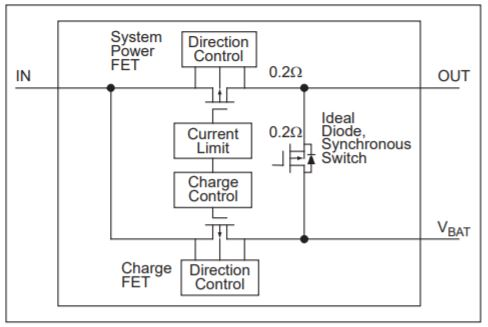
\includegraphics[scale=1.0]{figures/load-sharing.JPG}
    \caption{Load Sharing Design of the MCP73871.}
    \label{Sytem Load Sharing} 
\end{figure}
The second of the two Li-Io charge controllers researched was the MCP73871 stand-alone system load sharing and Li-Ion battery charge management controller. The MCP73871 chip is equipped with both AC-DC wall adapter and USB port power source selections, satisfying the design requirement for having two main sources available to power and charge the system. One of the most attractive features of the MCP73871 charge controller was its autonomous system load sharing feature. This allows the Aether node to be fully operational while simultaneously charging the Li-Io battery. Additionally, the charger automatically uses available input power to meet the system load demands, directly taking the input voltage to the output pin. In the situation where input power, whether it be solar or USB, does not meet the load demands, the charger draws the remaining current demand from the battery up to 1.8A. A Voltage Proportional Charge Controller or VPCC pin on the IC is used to prioritize the system load demands over the the Li-Io battery charge. This means the MCP73871 is constantly powering the system while the battery is being charged and discharged. A key improvement to the design of this solar/USB charger is a pass transistor inside the chip connected to the load output. This transistor prevents the loss of efficiency from charging and discharging the Li-Io battery.In \ref{fig:load-sharing} the interior design of MCP73871's load sharing is shown in more detail.    
\paragraph{}
The MCP73871 comes with a constant voltage regulation feature that is fixed with four available options depending on the charge requirements of the Li-Io battery: 4.10V, 4.20V, 4.35V or 4.40V. In conjunction with a thermistor, the charge controller is also able to regulate charge current depending on the temperature of the battery to ensure reliability and optimization of the system. In addition to these features, this solar/USB charge controller comes equipped with three battery status pin indicating a low battery state, charging done state, and a power on state. LED's can be connected to these pins to indicate to the user that status of the system and they can simultaneously be configured to a micro-controller to relay the information back to the server.     

\subsection{Batteries}
In this section, we provide an overview of the different types of batteries that we considered for use in our design. These types include lead acid batteries and lithium batteries. We also cover the different characteristics that we considered during the process of choosing a battery type.

\begin{figure}
    \centering
    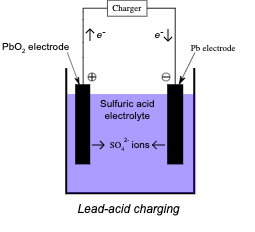
\includegraphics[scale=0.25]{figures/lead-acid-battery.png}
    \caption{The configuration of a lead acid battery.}
    \label{lead-acid-battery} 
\end{figure}

\subsubsection{Lead Acid Batteries}
Lead batteries consist of two electrodes, a negative electrode consisting of lead and a positive electrode consisting of a lead oxide. The two electrodes are submerged in an electrolyte solution comprised of a mixture of water and sulfuric acid. Typically, an electrically insulating material that is chemically permeable is added to ensure the two electrodes do not come into direct contact. The configuration of a lead acid battery can be seen in Figure \ref{lead-acid-battery}, while the chemical equation of the reaction being implemented can be found in Equation \ref{lead-acid-eqn}.

\begin{equation}
    \text{PbO}_2 + \text{Pb} + 2\text{H}_2\text{SO}_4
    \xLeftrightarrow[charge]{discharge}
    2\text{PbSO}_4 + \text{H}_2\text{O}
    \label{lead-acid-eqn}
\end{equation}

\subsubsection{Lithium Batteries}
Lithium batteries differ in a few substantial ways from their lead acid counterparts. The basic component of a lithium battery is a positively charged cathode typically made of a lithium oxide metal that will give off lithium ions. A negatively charged anode that while charging, will store lithium ions from the cathode and while discharging will allow the lithium ions flow through the electrolyte and the electrons through the electrical path back to the cathode. The Electrolyte is usually a material that is highly ionic conductive, this will permit lithium ions to pass through while the electrons will be kept in the anode. The last material is called the separator and it usually consists of polyethylene or polypropylene. The separators' job is to not inhibit the other functions of the battery but also keep the anode and cathode from coming into physical contact. The configuration of a lithium-ion battery can be found in Figure \ref{lithium-ion-battery}.

\begin{figure}
    \centering
    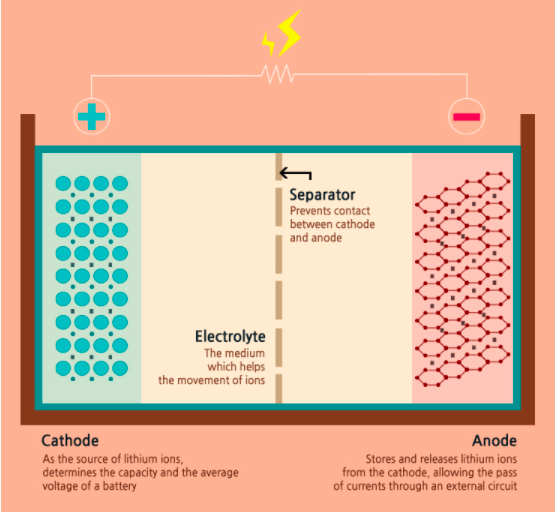
\includegraphics[scale=0.4]{figures/lithium ion battery.png}
    \caption{The configuration of a lithium ion battery.}
    \label{lithium-ion-battery} 
\end{figure}

\subsubsection{Battery Characteristics}
To utterly understand which battery is the right choice for a project one must look at how these methods of constructing a battery will affect the overall characteristics of the battery. The characteristics that impact the usefulness of a battery are as follows: discharge curve, energy density, temperature dependence, service life, charge/discharge cycle, and cost. Once we have amassed information around each characteristic we can then compare Lead acid to lithium batteries more thoroughly. From there if there is not an overall better choice in each and every category we will decide based on which characteristic is most important to complete the objectives of the project. For instance if it is determined that lithium would put us out of our needed price range but is only marginally better than lead acid in other categories then our overall decision will be impacted. Much like any well thought out purchase, we must look at each characteristic to gain a better understanding of how our project is being designed and where money is being allocated to.

\paragraph{Discharge Curve}
A discharge curve is a graph that plots Voltage against percentage of the capacity discharged. Essentially the Output voltage of a battery will lower as the battery is used up. Given this effect the most desirable curve would be flat (keeping voltage consistent at every level of discharge), so let us look at the average discharge curve of our lead acid and lithium-ion batteries. Figure \ref{fig:discharge-curve} shows example discharge curves one might find in a lithium ion and lead acid batteries. The figure has been provided by Power Tech, an energy storage system manufacturer. This figure shows first hand how steadily lead acid batteries drop in voltage as the depth of discharge increases. Meanwhile lithium is kept at a steady for the most part until the depth of discharge reaches upwards of 80 percent.

\begin{figure}
    \centering
    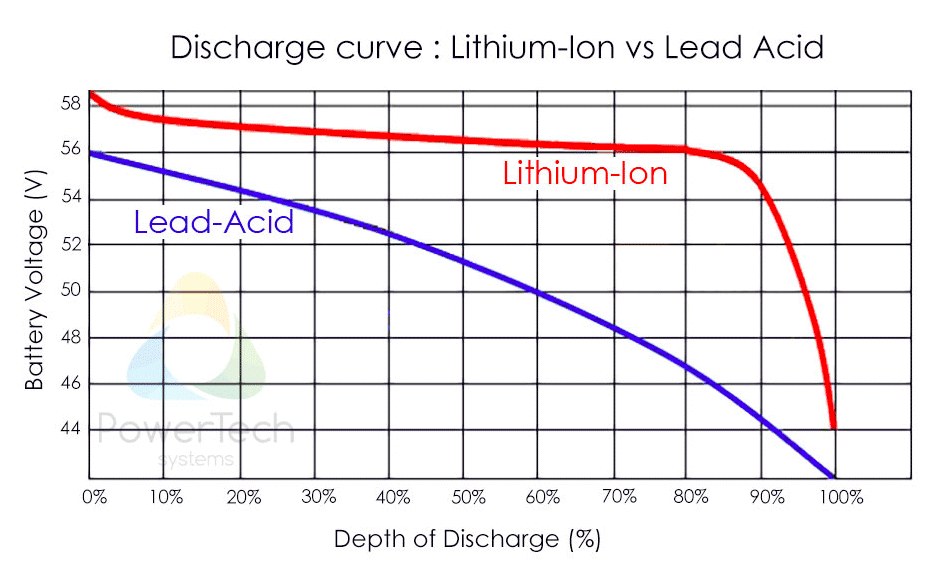
\includegraphics[scale=0.4]{figures/discharge curve.png}
    \caption{A comparison of a lithium ion battery discharge curve and a lead acid battery discharge curve.}
    \label{fig:discharge-curve} 
\end{figure}

\paragraph{Energy Density}
Energy density is the amount of energy you can get out of a battery per unit volume of weight required. Clearly the higher the density the better for a battery. The characteristic known as specific energy density is closely related. However, it considers the Discharge curve of the battery and how it would affect the voltage and current during the battery discharge cycle and is solely measured against weight. An example of the range of energy density and specific energy density can be found in Figure \ref{fig:energy-density} and is provided by the National Aeronautics and Space Administration. This figure shows that lithium far surpasses lead acid in energy density. When it comes to density by volume and density by weight lithium is roughly three times superior to lead acid.

\begin{figure}
    \centering
    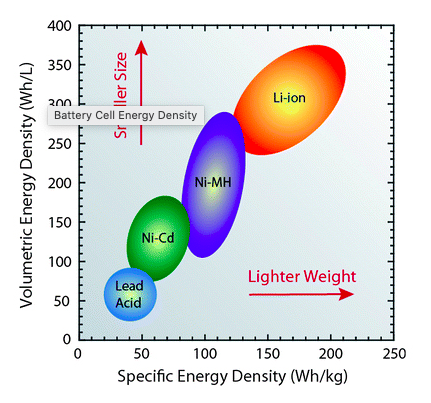
\includegraphics[scale=0.4]{figures/energy density.png}
    \caption{A comparison between volume energy density and specific energy density for various battery types.}
    \label{fig:energy-density} 
\end{figure}

\paragraph{Temperature Dependence}
Battery performance and temperature are highly correlated. Rates of reaction within battery cells themselves are temperature dependent as well as the internal resistance. Low temperatures give higher resistances in a battery, could freeze the electrolyte giving a lower voltage, and cause a steeper discharge curve. At higher temperatures chemicals may decompose or cause enough energy to become available to activate unintended reactions reducing the capacity. The temperature ranges for charging and discharging the viewed battery types are shower in Table \ref{tab:temperature-dependence}. This information came from Battery University(TM) an online free website teaching hands on battery information. This tables shows that the temperature ranges during charge and discharge are relatively similar with the only difference coming in charging advisories. As one can see lead acid is suited better below freezing during charging mean while lithium performs better at higher temperatures at the cost of its life span. 
\begin{table}
\centering\scriptsize
\caption{Temperature Dependence}
\begin{tabularx}{\linewidth}{|c|c|c|X|}
\hline
Battery Type & Charge Temperature & Discharge Temperature & Charge Advisory \\ 
\hline\hline

Lead Acid     & -20 C to 50 C   & -20 C to 50 C & Charge at 0.3 C or less below freezing Lower V-threshold by 3 mV/C when hot  \\\hline
Li-ion        & 0 C to 45 C     & -20 C to 60 C & No charge recommended below freezing. Good charge/discharge performance at higher temperature but shorter life.  \\\hline

\end{tabularx}
\label{tab:temperature-dependence}
\end{table}
\paragraph{Service Life}
As each recharge cycle of a rechargeable battery takes place its active components are slowly depleted, lowering its capacity. The industry service life of rechargeable batteries is defined as when the battery's capacity is 80\% of its intended use. The typical service life of rechargeable batteries could be anywhere from 500-1200 cycles. Figure \ref{fig:service-life} shows how repeated cycles influence the types of batteries were researching with the lead acid curve on the left and lithium ion on the right. As seen within the figure lithium batteries could go through 2-3 times the number of cycles as lithium batteries with a similar depth of discharge available.

\begin{figure}
    \centering
    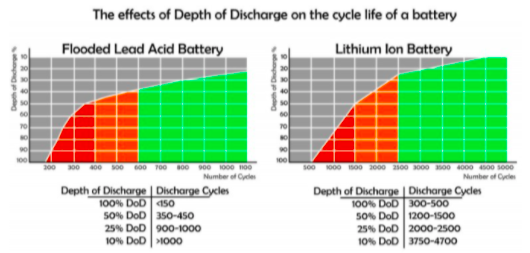
\includegraphics[scale=0.5]{figures/service life.png}
    \caption{A comparison between the service life of lead acid and lithium ion batteries.}
    \label{fig:service-life} 
\end{figure}

\paragraph{Charge Curve}
The charge curve shows the process of charging different batteries. This would include information on the voltage needed to charge, current used to charge, charging times, and capacity of battery. Figure \ref{fig:lead-acid-charge-curve} shows the charge curve for an example lead acid batteries provided by power sonic a battery manufacturer, and figure \ref{fig:lithium-charge-curve} shows the charge curve for an example lithium-ion battery from Battery University(TM) an online free website teaching hands on battery information. While the charging curves will differ from battery to battery meaning the examples are not completely accurate as to what can be expected the overall structure of the curve will match those with similar chemistry. What we can see reliably however are a the charging time for lithium batteries are far lower than their lead acid counter parts.

\begin{figure}
    \centering
    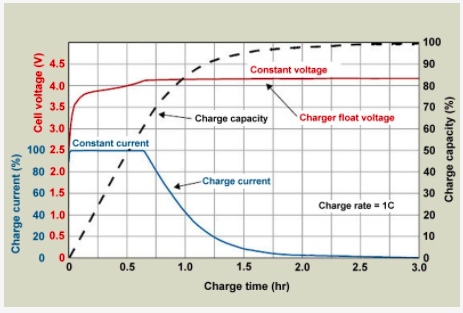
\includegraphics[scale=0.5]{figures/lithium charge curve.png}
    \caption{The charge curve for a lithium ion battery.}
    \label{fig:lithium-charge-curve} 
\end{figure}

\begin{figure}
    \centering
    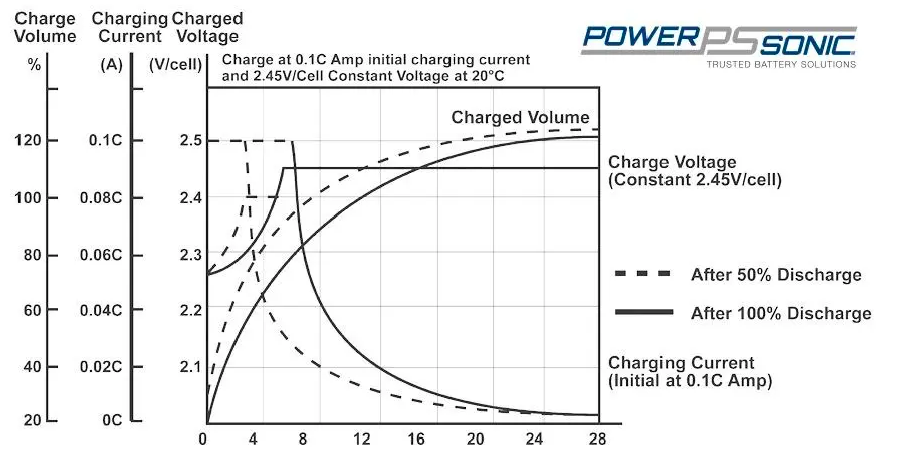
\includegraphics[scale=0.5]{figures/lead acid charge curve.png}
    \caption{The charge curve for a lead acid battery.}
    \label{fig:lead-acid-charge-curve} 
\end{figure}
\paragraph{Cost}
The cost category is self-explanatory. When it comes down to the devices components certain materials can be acquired for a much lower cost than others. For example, according to the US government in 2018 lithium costs \$13,000 per metric ton, while on the other hand during the same year lead hit an all-time high with \$2,600 per metric ton. Table (b) is a handy chart to estimate the cost one could expect to pay for the batteries we have researched. Information within the table comes from "Off Grid Solar: a handbook for Photovoltaics with Lead-Acid and Lithium-Ion batteries" by Joseph P. O'Conner.

\begin{table}
\centering\scriptsize
\caption{Initial cost per capacity and cost per life cycle comparison between lead acid and lithium ion batteries.}
\begin{tabular}{|r|c|c|}
\hline
& Flooded Lead Acid & Lithium-Ion \\ 
\hline
Initial Cost per Capacity (USD/kWh)    & 131   & 530  \\\hline
Cost per Life Cycle (USD/kWh)    & 0.17     & 0.19 \\\hline
\end{tabular}
\label{tab:battery-cost-comparison}
\end{table}

Throughout this section, we have researched and explored the different characteristics that impact how a specific type of battery functions. Here we will provide a provide a brief summary of the comparison of the battery characteristics between lithium ion batteries and lead acid batteries. The overall discharge curve of lithium batteries is much flatter than lead acid, indicating that they give a constant voltage as they discharge. In terms of materials, lithium ion batteries have a much higher energy density than lead acid batteries meaning that the batteries will be smaller, weigh less, and have a higher capacity.  In terms of temperature change, lead acid batteries have a higher temperature range and vice versa for discharge and lithium ion batteries. The charging advisory for lithium ion batteries is higher and not supposed to occur below freezing, which can be an issue in colder climates. We can see the depth of discharge has a much steeper curve for lead acid batteries. This tells us that lithium ion batteries can go through more charge cycles before becoming reaching the 80\% capacity threshold. The only large difference in the charge curve between lead acid batteries and lithium ion batteries is that lithium ion batteries have a much shorter charge time. Finally, the comparison between initial cost per capacity and cost per life cycle between both battery types can be observed in Table \ref{tab:battery-cost-comparison}. The operational cost per cycle is slightly higher and the upfront cost is much higher for lithium ion batteries. Due to these factors we have decided to use a lithium ion battery in our design.

\subsubsection{Summary}
Throughout this section we have noticed many large and small differences between our possible selections. These have been complied and are presented as such in table (c). You can plainly see when compared lithium ion out performs lead acid in terms of quality however in terms of cost lead acid clearly leads. As a result our project must choose if lithium acids' quality exceeds the increase in price tag and it has been decided that it has. As a result of sing a lithium ion battery our project will be better equipped in colder climates, last longer, and give a more constant output during use. 
\begin{table}
\centering\scriptsize
\caption{Differences between Lead Acid and Lithium Ion Batteries}
\begin{tabular}{|r|c|c|}
\hline
Characteristic&Findings \\\hline

Discharge Curve&The overall discharge curve of lithium was much flatter showing that they give a constant voltage as they discharge. 
  \\\hline
Energy Density&In terms of materials lithium has a much higher energy density than lead meaning that the batteries will be smaller, weigh less, and have a higher capacity. 
  \\\hline
Temperature Dependence&When it's come to temperature charge lead acid has a higher temperature range and vice versa for discharge and lithium. Charging advisory for lithium is higher and not supposed to occur below freezing which can be a factor in colder climates. 
  \\\hline
Service Life&As we can see the depth of discharge has a much steeper curve for lead acid. This tells us that lithium can go through more charge cycles before becoming reaching the 80% capacity threshold. 
  \\\hline
Charge Curve&The only large difference in the charge curve is lithium's much shorter charge time.  
Cost&The cost of lead acid and lithium are clear and square from the table. The operational cost per cycle is slightly higher and the upfront cost is much higher.
  \\\hline
\end{tabular}
\label{tab:battery-comparison}
\end{table}

\paragraph{Decision}
The chosen battery is the PRT-13856. This is a 3 cell battery with a voltage of 3.7V and 6AH. This means we can expect 22.2WH of capacity allowing our device to run for months without need of ever recharging. This battery will be a major asset when it comes to concerns of keeping our system supplied with power in more extreme conditions over longer periods of time. A link to the data sheet is as follows:
https://www.digikey.com/en/products/detail/sparkfun-electronics/PRT-13856/6605200

\subsection{Solar Panel}

\begin{figure}
    \centering
    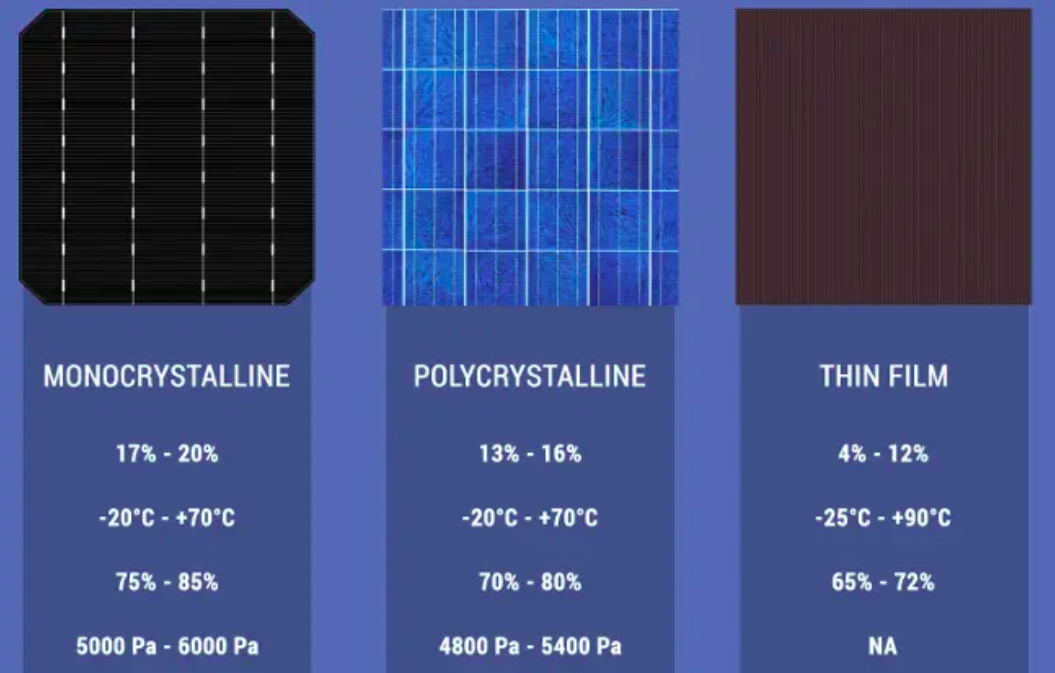
\includegraphics[scale=0.4]{figures/solar panel overview.png}
    \caption{The three types of solar panels.}
    \label{solar-panel-overview} 
\end{figure}

In this section, we will discuss the different types of solar panels that are being considered for use in our design. Discovered in the early 19th century solar panels utilize the photovoltaic effect. This phenomenon was observed when certain materials were produced and electric current when exposed to light. The way this phenomenon is utilized by using two semiconducting materials. One layer must have depleted electrons and when exposed to sunlight some photons are absorbed by the semiconductor which excites the electrons causing them to jump from one semiconductor layer to another. This jump produces a small electric current which when happens in mass makes a usable power source. The most common material to use in solar panels is silicon which is cut and polished into wafers. Some of these wafers are doped to make an electrical imbalance further helping the process. Finally, electrically conductive strips are attached to the cells to absorb the generated current. 

\subsubsection{Monocrystalline Solar Panels}

Like the name suggests monocrystalline solar panel cells are made from a single crystal of silicon. Having a single crystal gives electrons more room to flow providing greater efficiency providing more power to the load which is the largest advantage of this type of panel. This, however, is more difficult to create, making it the more expensive option. This structure also provides more durability enabling the panel to last for years longer than its alternatives. An example of the features one can expect from a monocrystalline panel can be seen in Figure \ref{fig:mono-sp}. Here one can see the EVA films on either side of the silicon wafers. The wafers itself made up of a single bar of silicon giving the solar panel its name monocrystaline. This figure was provided by Alternative Energy Solutions, as alternative energy information source.

\begin{figure}
    \centering
    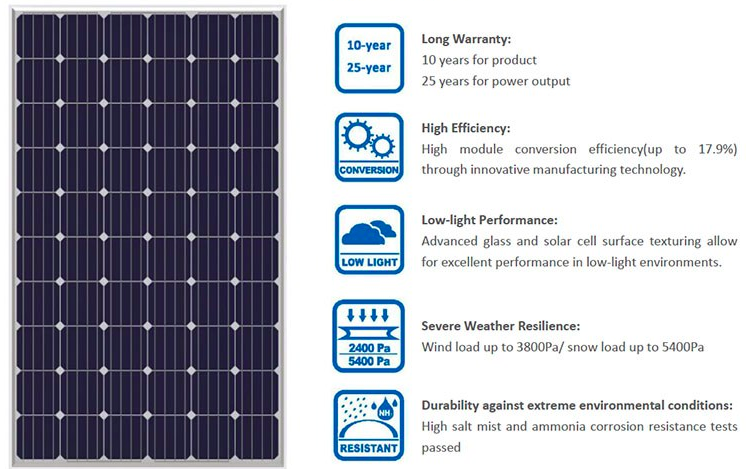
\includegraphics[scale=0.5]{figures/monocrystaline.png}
    \caption{An example of a monocrystaline solar panel.}
    \label{fig:mono-sp} 
\end{figure}
\subsubsection{Polycrystalline Solar Panels}

Unlike monocrystalline panels these solar panel cells are made from many crystals of silicon. This offers much less freedom of movement for electrons which gives a much higher efficiency. This is also simpler to build, meaning that costs are lower, which could be a factor in our decision. This structure also provides not as much durability as its monocrystalline counterpart however it does last longer than its thin film competition. An example of the features one can expect from a polycrystalline panel can be seen in Figure \ref{fig:poly-sp}. Here one can see the EVA films on either side of the silicon wafers. The wafers itself made up of silicon fragments melted together to produce individual wafers giving the solar panel its name polycrystalline. This figure was provided by Clean Energy Reviews an independent energy source review site.

\begin{figure}
    \centering
    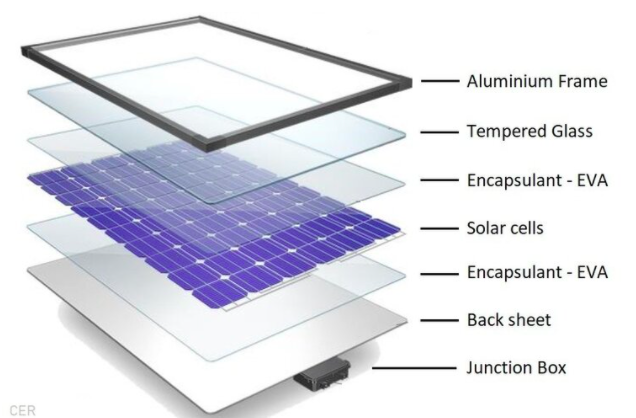
\includegraphics[scale=0.4]{figures/polycrystaline solar.png}
    \caption{Polycrystaline Solar Panel.}
    \label{fig:poly-sp} 
\end{figure}
\subsubsection{Thin Film Solar Panels}

Unlike the previous two types of solar panels, thin film solar panels are mostly not made of silicon. They are made of a mixture of materials mostly cadmium telluride, which is comprised into a thin sheet between two transparent conductive layers that help capture sunlight. Thin film solar panels usually have the lowest efficiency and durability of all solar panel types however they make up for it in flexibility and where it can be comfortably placed . The main advantage of this type of solar panel is their low weight, profile, and its ability to adhere to whatever required surface it may need to. Figure \ref{fig:thin-film-sp} shows an example of thin film solar panels. This figure was provided by Sun Power Source, a solar energy review, news, and project work site.
\begin{figure}
    \centering
    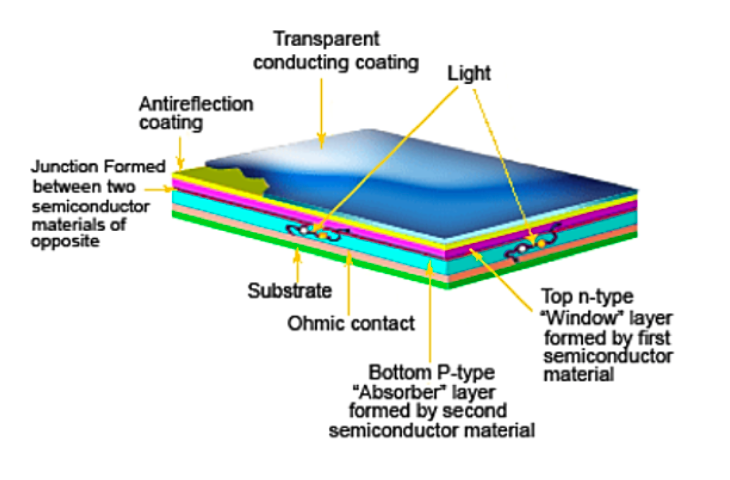
\includegraphics[scale=0.4]{figures/thin film solar.png}
    \caption{An example of a thin film solar panel.}
    \label{fig:thin-film-sp} 
\end{figure}

\subsubsection{Summary}
\begin{table}
\centering\scriptsize
\caption{Differences between Solar Panel Subtypes}
\begin{tabular}{|r|c|c|}
\hline
&Efficiency(percent)&Cost(Price Per Watt(USD))&Projected Life Span(Years) \\\hline

MonoCrystaline&17-20&1.00-1.50&25-35\\\hline

PolyCrystaline&13-16&0.70-1.00&23-27\\\hline

Thin-Film&4-12&1.00-1.50&14-17\\\hline
\end{tabular}
\label{tab:Solar-Panel-comparison}
\end{table}

The selection of solar panels comes down to less factors than the battery. Here the differences between the first two types monocrystaline and poly crystaline are very straight forward. Monocrystaline will provide more efficiency and durable but polycrystaline will be more affordable. However when thin film solar panel are introduced we must consider different factors such as placement of the solar panel. Show we provide the solar panel with a jagged or uneven surface to be placed on then extra precautions would be needed to have one of the first two panels making thin film more convenient and reliable. How ever due to the nature of our project and its intended use we can comfortably provide our solar panel with a reliable and safe solar panel placement leading once again if the increase in efficiency is worth the increase in cost, the increase in cost being roughly 20 percent on average given the typical cost. Seeing as on average monocrystaline is between 6 and 53 percent more efficient with the average being 20 percent more efficient than polycrystaline our team has decided that the increase in cost is justified. As a result the solar panel we have decided upon is the P105, a monocrystaline 5.5W 6V solar panel. This should provide our system with a reliable and powerful source of power capable of keeping the system independently online.


\subsection{USB Power}
In our design we wish to plan for a scenario in which a field crew could come and charge the battery quickly and keep basic nodal functions operational without the need to wait for a solar panel. This functionality could also come in handy if certain equipment were to malfunction discontinuing the capabilities of the node to recharge itself. As such a design has been implemented as seen in Figure X. This design incorperates an IC that receives power from the solar panel and a USB charging connection. The circuit would take power from the solar panel and feed it to the load and battery, unless the input selection pin were instructed to take power from the USB connection and use that to power the load and charge the battery. This way the battery could take in power from either only the solar panel or USB connection.
